\section*{VADER (5 pts)}

\section*{Q1: Workings of VADER}

According to VADER’s repository \cite{vader}, VADER (Valence Aware Dictionary and sEntiment Reasoner) is a rule-based sentiment analysis tool which uses a combination of lexicon-based and rule-based approaches to determine the sentiment polarity of a given text, and is especially designed for analyzing social media texts.

VADER uses a pre-built lexicon of words (validated by human raters) that have associated ‘valence’ scores: for each text, we find the words within that text that belong to the lexicon, sum their valence scores, adjust to VADER’s rules, and normalize to range between -1 and 1. This gives the compound score of the whole text, which we then threshold to get a ternary classification: positive, negative, or neutral.


\section*{Q2: Code}

Code snippet \cref{listing:p2-code1} shows how we have used VADER for our use case. The lexicon that VADER uses is especially suitable for social media, and thus, there is no need to tokenize tweets and remove stopwords. However, it is still important to preprocess the tweet strings into clean text (by the methods shown in code snippet \cref{listing:p1-code1}).

\begin{listing*}
\begin{minted}{python}
from vaderSentiment.vaderSentiment import SentimentIntensityAnalyzer
sid_obj = SentimentIntensityAnalyzer()

def map_sentiment(compound_val):
   if compound_val >= 0.05:
       return 'positive'
   if compound_val <= - 0.05:
       return 'negative'
   else:
       return 'neutral'
df_tweets['vader_polarity'] = [sid_obj.polarity_scores(sentence) for sentence in df_tweets['TweetText']]
df_tweets['vader_decision'] = [map_sentiment(sentiment_dict['compound']) for sentiment_dict in df_tweets['vader_polarity']]

# convert our dataset to positive, negative and neutral labels by adding pos_sent and neg_sent
df_tweets['overall_sent_GT'] = df_tweets['pos_sent'].astype('int') + df_tweets['neg_sent'].astype('int')
def map_int(val):
   if val > 0:
       return 'positive'
   if val < 0:
       return 'negative'
   else:
       return 'neutral'
df_tweets['overall_sent_GT'] = [map_int(val) for val in df_tweets['overall_sent_GT']]

from sklearn.metrics import confusion_matrix
confusion_matrix(df_tweets['overall_sent_GT'], df_tweets['vader_decision'])
\end{minted}
\caption{Using VADER for our dataset, and converting our labels to three classes to measure the performance of VADER.}
\label{listing:p2-code1}
\end{listing*}


\section*{Q3: Application to TweetsCOV19 dataset, Performance}

We convert our ground truth labels into VADER-compatible labels by summing the positive and negative values, and taking the sign of the output. If the value is 0, it is neutral. While this approach is straightforward, it is quite naive (for example, a tweet that is labeled as (5, -5) classified as neutral in the same manner as a tweet labeled as (1, -1)). However, since extreme tweets (whose sentiment is higher than 3 for either positive or negative sentiments) are quite rare in the dataset, and there is no other straightforward heuristic for conversion, we choose this naive solution.

In Figure \ref{fig:vader}, we plot our confusion matrix between our VADER-converted ground truth labels, and the VADER predictions. 

\begin{figure}
    \centering
    \begin{subfigure}{0.49\columnwidth}
        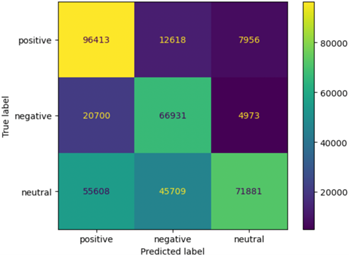
\includegraphics[width=1\textwidth]{images/vader_conf.png}
    \end{subfigure}
    \centering
    \begin{subfigure}{0.49\columnwidth}
        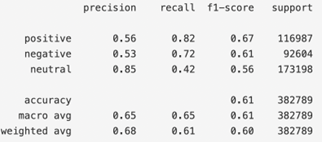
\includegraphics[width=1\textwidth]{images/vader_class.png}
    \end{subfigure}
    \caption{Confusion matrix and classification report of VADER’s predictions on the basis of our converted ground truth labels.}
    \label{fig:vader}
\end{figure}

While the performance evaluation of the VADER method might not seem impressive, it is important to remember that our ground truth labels are not adapted to the ternary classification task, and thus it is unwise to cast doubts on VADER’s predictions on this basis. Furthermore, the F1-score of every class is between 56\% and 67\%, and while these are not very high figures, they do show some agreement between our ground truth labels and the VADER method.
